\documentclass[reqno]{amsart}
\usepackage{amscd, amssymb, amsmath, amsthm}
\usepackage{graphicx}
\usepackage[colorlinks=true,linkcolor=blue]{hyperref}
\usepackage[utf8]{inputenc}
\usepackage[T1]{fontenc}
\usepackage{textcomp}
\usepackage{babel}
%% for identity function 1:
\usepackage{bbm}
%%For category theory diagrams:
\usepackage{tikz-cd}
\usepackage{enumitem}


\setlength\parindent{0pt}

\pdfsuppresswarningpagegroup=1

\newtheorem{theorem}{Theorem}[section]
\newtheorem{lemma}[theorem]{Lemma}
\newtheorem{proposition}[theorem]{Proposition}
\newtheorem{corollary}[theorem]{Corollary}
\newtheorem{conjecture}[theorem]{Conjecture}

\theoremstyle{definition}
\newtheorem{definition}[theorem]{Definition}
\newtheorem{example}[theorem]{Example}
\newtheorem{exercise}[theorem]{Exercise}
\newtheorem{problem}[theorem]{Problem}
\newtheorem{question}[theorem]{Question}

\theoremstyle{remark}
\newtheorem*{remark}{Remark}
\newtheorem*{note}{Note}
\newtheorem*{solution}{Solution}



%Inequalities
\newcommand{\cycsum}{\sum_{\mathrm{cyc}}}
\newcommand{\symsum}{\sum_{\mathrm{sym}}}
\newcommand{\cycprod}{\prod_{\mathrm{cyc}}}
\newcommand{\symprod}{\prod_{\mathrm{sym}}}

%Linear Algebra

\DeclareMathOperator{\Span}{span}
\DeclareMathOperator{\Ima}{Im}
\DeclareMathOperator{\diag}{diag}
\DeclareMathOperator{\Ker}{Ker}
\DeclareMathOperator{\ob}{ob}
\DeclareMathOperator{\Hom}{Hom}
\DeclareMathOperator{\sk}{sk}
\DeclareMathOperator{\Vect}{Vect}
\DeclareMathOperator{\Set}{Set}
\DeclareMathOperator{\Group}{Group}
\DeclareMathOperator{\Ring}{Ring}
\DeclareMathOperator{\Ab}{Ab}
\DeclareMathOperator{\Top}{Top}
\DeclareMathOperator{\hTop}{hTop}
\DeclareMathOperator{\Htpy}{Htpy}
\DeclareMathOperator{\Cat}{Cat}
\DeclareMathOperator{\CAT}{CAT}
\DeclareMathOperator{\Cone}{Cone}
\DeclareMathOperator{\dom}{dom}
\DeclareMathOperator{\cod}{cod}
\DeclareMathOperator{\Aut}{Aut}
\DeclareMathOperator{\Mat}{Mat}
\DeclareMathOperator{\Fin}{Fin}
\DeclareMathOperator{\rel}{rel}
\DeclareMathOperator{\Int}{Int}
\DeclareMathOperator{\sgn}{sgn}

%Row operations
\newcommand{\elem}[1]{% elementary operations
\xrightarrow{\substack{#1}}%
}

\newcommand{\lelem}[1]{% elementary operations (left alignment)
\xrightarrow{\begin{subarray}{l}#1\end{subarray}}%
}

%SS
\DeclareMathOperator{\supp}{supp}
\DeclareMathOperator{\Var}{Var}

%NT
\DeclareMathOperator{\ord}{ord}

%Alg
\DeclareMathOperator{\Rad}{Rad}
\DeclareMathOperator{\Jac}{Jac}

%Misc
\newcommand{\SL}{{\mathrm{SL}}}
\newcommand{\mobgp}{{\mathrm{PSL}_2(\mathbb{C})}}
\newcommand{\id}{{\mathrm{id}}}
\newcommand{\Mod}{{\mathrm{Mod}}}
\newcommand{\ud}{{\mathrm{d}}}
\newcommand{\Vol}{{\mathrm{Vol}}}
\newcommand{\Area}{{\mathrm{Area}}}
\newcommand{\diam}{{\mathrm{diam}}}


\newcommand{\reg}{{\mathtt{reg}}}
\newcommand{\geo}{{\mathtt{geo}}}

\newcommand{\tori}{{\mathcal{T}}}
\newcommand{\cpn}{{\mathtt{c}}}
\newcommand{\pat}{{\mathtt{p}}}




\begin{document}
\section{Curves, Surfaces and Hyperbolic Geometry}
\subsection{Simple closed curves}
There is a bijective correspondence
\[
\left\{ 
    \begin{tabular}{c}
    Nontrivial\\
    conjugacy classes\\
    in $\pi_1 (S)$
\end{tabular}
\right\} 
\longleftrightarrow
\left\{ 
    \begin{tabular}{c}
        Nontrivial free\\
        homotopy classes of oriented\\
        closed curves in $S$
\end{tabular}
\right\} 
\] 

\begin{definition}[Primitive and multiple elements]
    An element $g$ of a group $G$ is \textit{primitive} if there
    does not exist any $h \in G$ so that $g = h^{k}$ for
    $\left| k \right| >1$. The property of being a primitive
    is a conjugacy class invariant. In particular, it makes
    sense to say that a closed curve in a surface is primitive.\\
    A closed curve in $S$ is a multiple if it is a map
    $S^{1} \to S$ that factors through the map
    $S^{1} \stackrel{\times n}{\to } S^{1}$ for
    $n >1$, i.e., there exists a map $\tilde{\alpha} \colon
    S^{1} \to S$ such that the following diagram commutes:
    \begin{equation*}
    \begin{tikzcd}
        S^{1} \ar[r, "\times n"] \ar[rr, bend left = 45, dashed,
        "\tilde{\alpha}"] & S^{1} \ar[r,
        "\alpha"] & S
    \end{tikzcd}
    \end{equation*}
\end{definition}

\begin{definition}[Lifts]
    We make a distinction between lifts: let $p \colon
    \tilde{S} \to S$ be a covering space. By a \textit{lift} of a closed
    curve $\alpha$ to $\tilde{S}$ we will always mean the image of
    a lift $\mathbb{R} \to \tilde{S}$ of the map
    $\alpha \circ \pi$ where $\pi \colon \mathbb{R} \to S^{1}$ is
    the usual covering map. I.e., a lift of $\alpha \colon
    S^{1} \to S$ is a map  $\tilde{\alpha} \colon \mathbb{R} \to 
    \tilde{S}$ such that the following diagram commutes
    \begin{equation*}
    \begin{tikzcd}
        & & \tilde{S} \ar[d, "p"]\\
        \mathbb{R} \ar[r, "\pi"'] \ar[rru, "\tilde{\alpha}"] & S^{1} \ar[r, 
        "\alpha"'] & S
    \end{tikzcd}
    \end{equation*}
    A lift is different from a \textit{path lift} which is
    a proper subset of a lift. Namely, it would be
    the restriction of $\tilde{\alpha}$ to some interval of
    $\mathbb{R}$ of length $2 \pi$ if the covering map
    $\pi$ is of the form $t \mapsto e^{it}$.
\end{definition}

Now suppose $p \colon \tilde{S} \to S$ is the universal cover
and $\alpha$ is a simple closed curve in $S$ that is
not a multiple of another closed curve. In this case, there
is a bijective correspondence
between cosets in $ \pi_1 (S)$
 of the infinite cyclic subgroup $\left<\alpha \right>$ and
 the lifts of $\alpha$. This can be seen as follows: first choose
 a basepoint $\alpha(1) =  x_0 \in S$
and
 some $\tilde{x_0} \in p^{-1}(x_0)$. There exists a unique lift
 $\tilde{\alpha}$ of $\alpha$ such that
 \begin{equation*}
 \begin{tikzcd}
     & & \tilde{S}\ar[d, "p"] \\
     \mathbb{R} \ar[r] \ar[rru, "\tilde{\alpha}"] & S^{1} \ar[r, "\alpha"] & S
 \end{tikzcd}
 \end{equation*}
 commutes and such that
 $\tilde{\alpha}(0) = \tilde{x} \in p^{-1}(\alpha \circ \pi (0))$
 for some specific $\tilde{x}$  \cite[Cor. 4.2]{Bredon}.
 But the set
 $p^{-1} \left( \alpha \circ \pi (0) \right) $ is in bijective
 correspondence with the loops in $\pi_1 (S)$ by the path lifting lemma. 
 Now, under which path lifts are the lifts the same? The lifts of
 $\alpha$ to two points $\tilde{x}, \tilde{y} \in 
 p^{-1}\left( \alpha \circ \pi (0) \right) $ will be the same if
 $\alpha^{k} \cdot \tilde{x} = \tilde{y}$ where
 $\cdot $ denotes the monodromy action of $\pi_1 (S)$ on
 the fiber. Now, there exist $\gamma_x$ and
 $\gamma_y$ in $\pi_1 (S)$ such that
 $\gamma_x \cdot \tilde{x_0} = \tilde{x}$ and
 $\gamma_y \cdot \tilde{x_0} = \tilde{y}$, so
 $\alpha^k \gamma_x = \gamma_y$. Hence the lifts
 corresponding to $\gamma_x$ and $\gamma_y$ are the same if and only
 if $\alpha^k \gamma_x = \gamma_y$ for some $k$, i.e. if and only if
 $\gamma_x = \gamma_y$ in $\pi_1(S) / \left<\alpha \right>$.\\
 \linebreak
 As usual, the group $\pi_1 (S)$ acts on the set of lifts
 of $\alpha$ by deck transformations, and this action agrees
 with the usual left action of $\pi_1 (S)$ on the
 cosets of $\left<\alpha \right>$. The stabilizer of the lift
 corresponding to the coset $\gamma \left<\alpha \right>$ is
 the cyclic group $\left<\gamma \alpha \gamma^{-1} \right>$. See
 figure~\ref{fig:lifts-of-paths}.

 \begin{figure}[http]
     \centering
     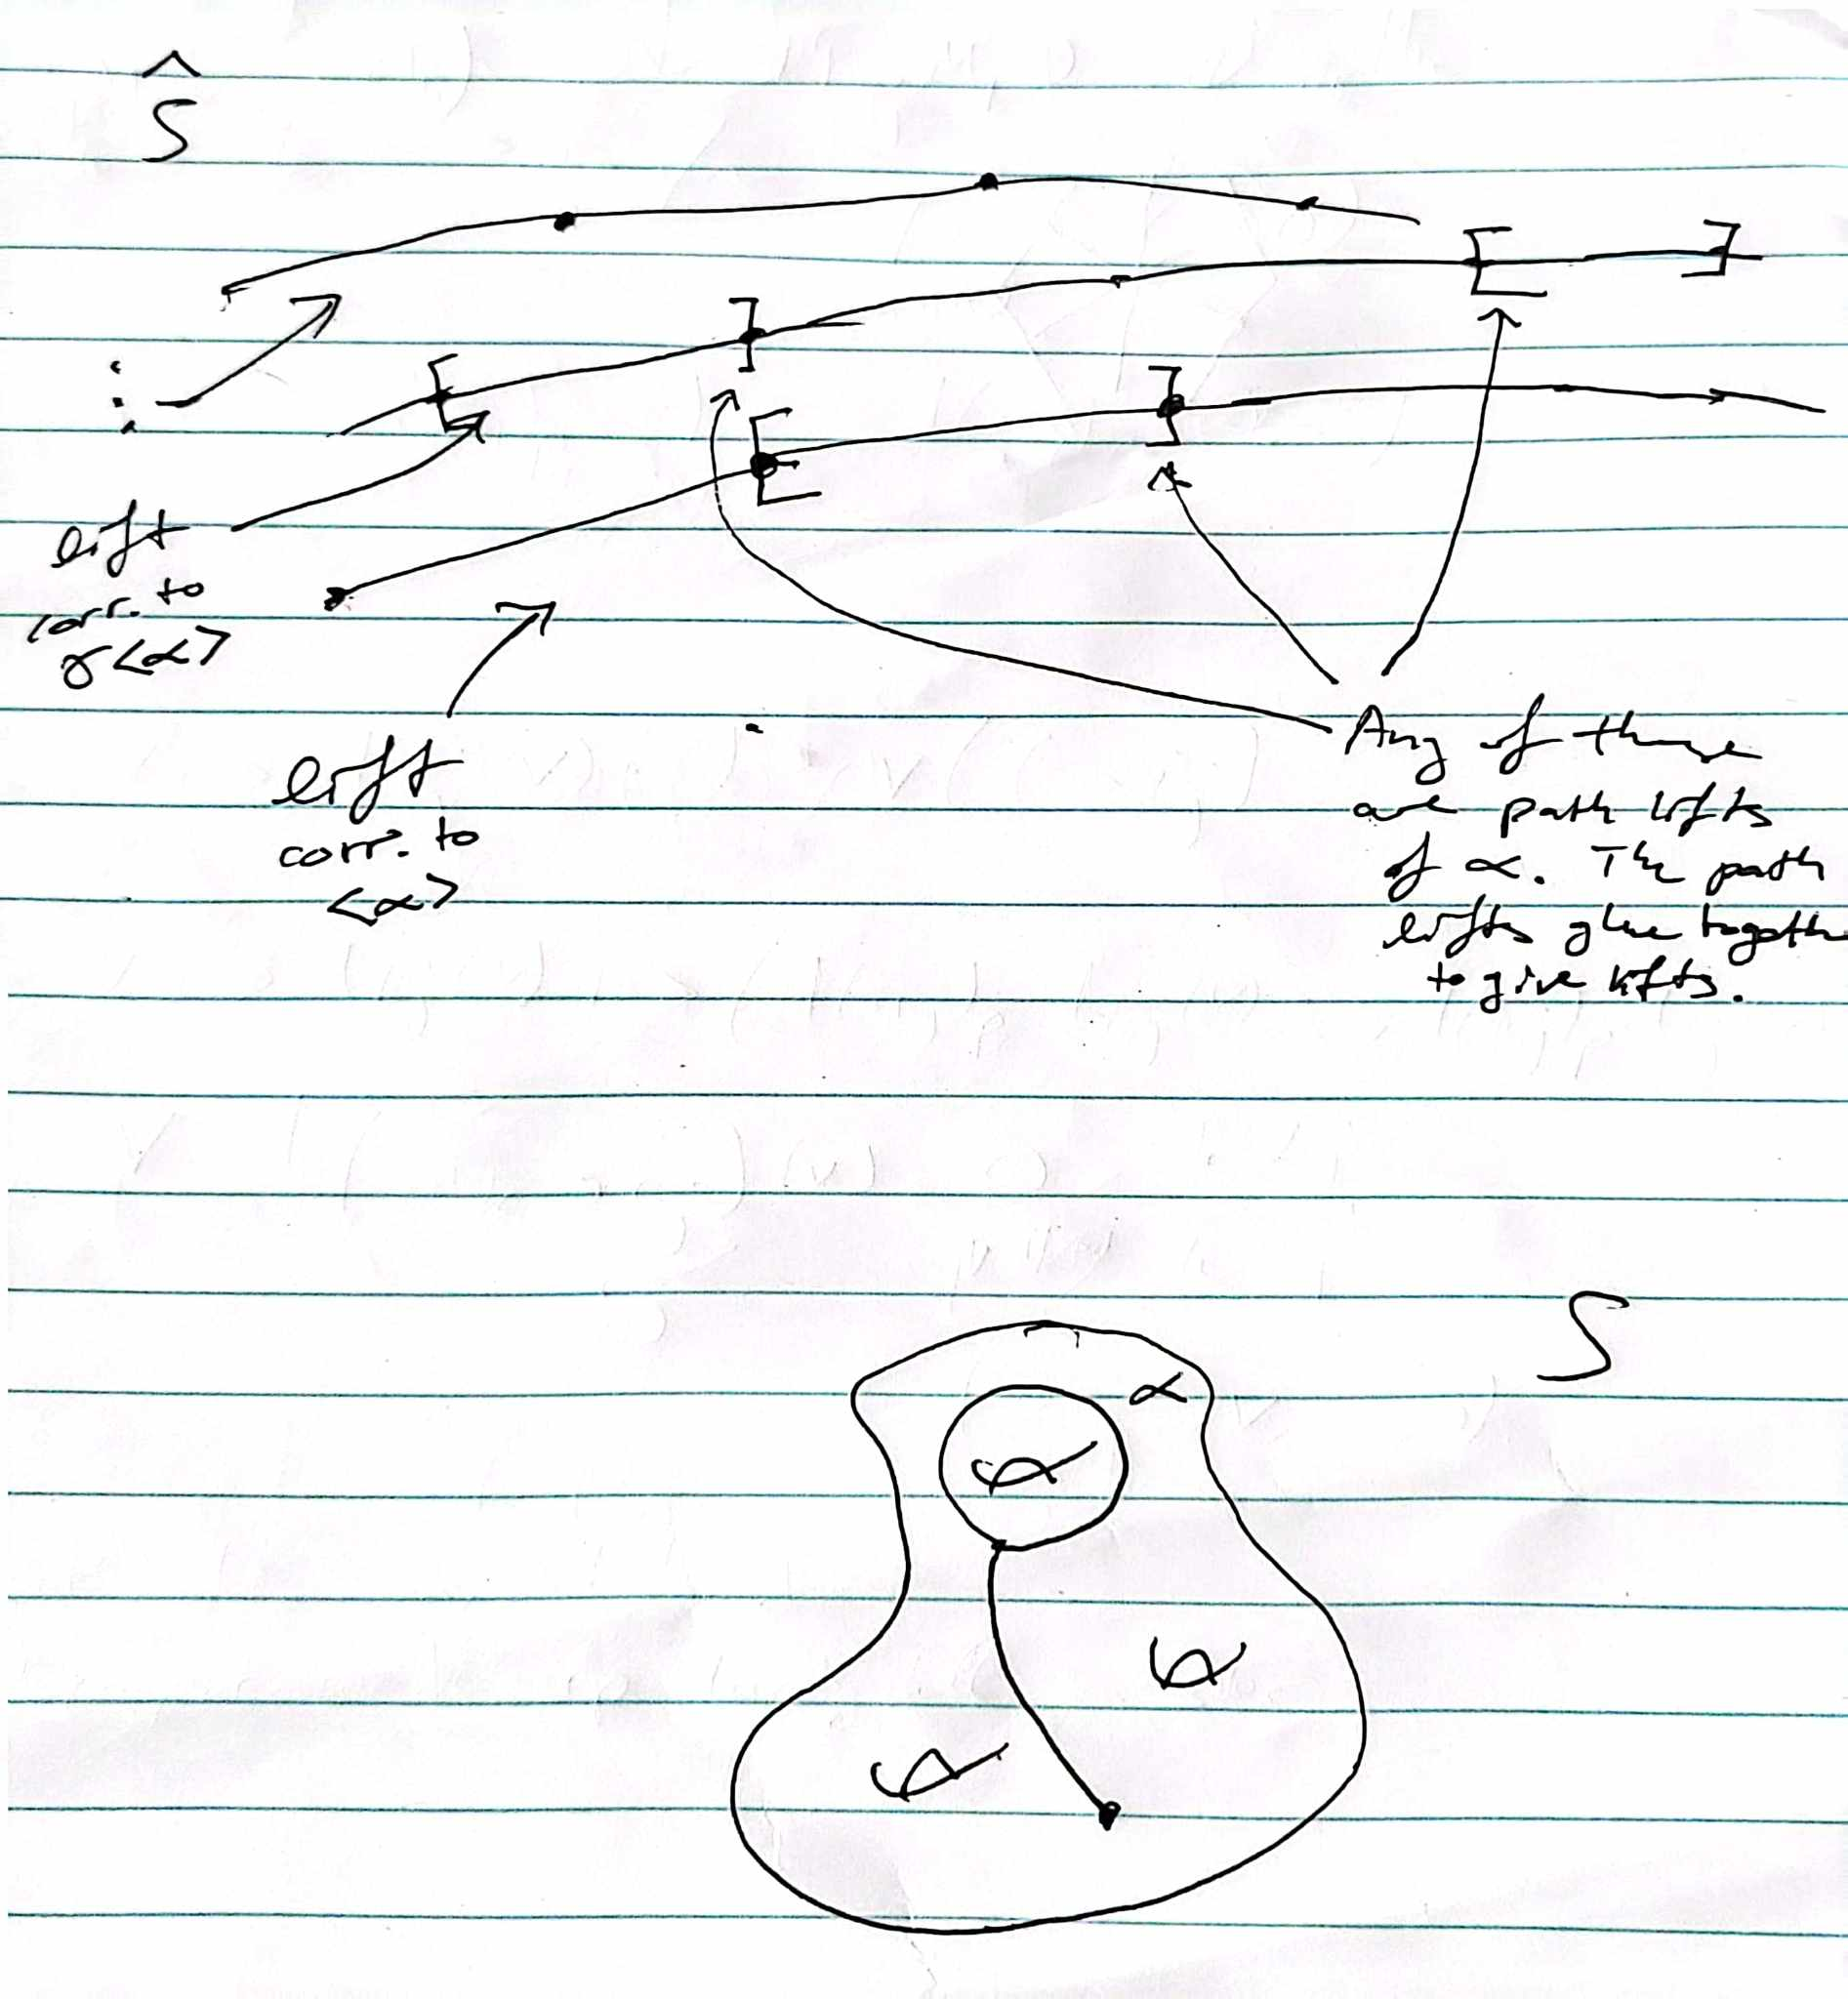
\includegraphics[width=0.8\textwidth]{lifts-of-paths.jpg}
     \caption{}
     \label{fig:lifts-of-paths}
 \end{figure}

 \begin{theorem}[]
When $S$ admits a hyperbolic metric and
$\alpha$ is a primitive element of $\pi_1 (S)$, we have
a bijective correspondence
\[
\left\{ 
    \begin{tabular}{c}
    Elements of the conjugacy\\
    class of $\alpha$ in $\pi_1 (S)$
\end{tabular}
\right\} 
\longleftrightarrow
\left\{ 
    \begin{tabular}{c}
    Lifts to $\tilde{S}$ of the\\
    closed curve $\alpha$
\end{tabular}
\right\} 
\] 


More precisely, we claim that the map which sends the lift
given by the coset $\gamma \left<\alpha \right>$ to
$\gamma \alpha \gamma^{-1}$ is bijective and well-defined.\\
 \end{theorem}

 \begin{proof}
To show that it is well-defined, suppose $\gamma \left<\alpha \right>$ and
$\beta \left<\alpha \right>$ give the same lift. Then
$\gamma = \beta \alpha^k$. So in particular,
\[
    \gamma \alpha \gamma^{-1} = \beta \alpha^k \alpha \alpha^{-k} \beta^{-1}
    = \beta \alpha \beta^{-1}
\] 
so they do correspond to the same element of the conjugacy class
$\left[ \alpha \right] $. It is clear that this is a surjective map.
Now suppose that $\gamma \alpha \gamma^{-1} = \beta \alpha \beta^{-1}$. 
Then $\beta^{-1} \gamma \alpha \left( \beta^{-1} \gamma \right)^{-1} =
\alpha$, so in particular, $\beta^{-1} \gamma \in C_{\pi_1(S)}(\alpha)$
which is a cyclic group generated by, say, $\theta$. But then
$\theta^l = \alpha$ since $\alpha$ is trivially in the centralizer of
$\alpha$; however, $\alpha$ is primitive, so
$l$ must be $\pm 1$, but then  $\alpha$ generates the centralizer of
$\alpha$, $C_{\pi_1 (S)}(\alpha) = \left<\alpha \right>$, and hence
$\gamma = \beta \alpha^l$, so $\gamma \left<\alpha \right>
= \beta \left<\alpha \right>$.
 \end{proof}

 \begin{remark}[]
     If $\alpha$ is any multiple, then we still have a bijective correspondence
     between elements of the conjugacy class of $\alpha$ and the
     lifts of $\alpha$. However, if $\alpha$ is not primitive and not
     a multiple, then there are more lifts of $\alpha$ than there
     are conjugates. Indeed, if $\alpha = \beta^{k}$, where $k > 1$, then
     $\beta \left<\alpha \right> \neq \left<\alpha \right>$ while
     $\beta \alpha \beta^{-1} = \alpha$.
 \end{remark}

 \begin{example}[]
     The above correspondence does not hold for the torus $T^2$ because
     each closed curve has infinitely many lifts, while
     each element of $\pi_1 \left( T^2 \right) \approx \mathbb{Z}^2$ 
     is its own conjugacy class because $\pi_1 \left( T^2 \right) $ is
     abelian. 
 \end{example}

 \subsubsection*{Geodesic representatives}
 \begin{proposition}[]\label{unique-geodesic-representative}
     Let $S$ be a hyperbolic surface. If $\alpha$ is a closed curve
     in $S$ that is not homotopic into a neighborhood of a puncture, then
     $\alpha$ is homotopic to a unique geodesic closed curve $\gamma$.
 \end{proposition}
 
 \begin{corollary}
     For compact hyperbolic surfaces, 
     there is a bijective correspondence:
\[
\left\{ 
    \begin{tabular}{c}
        Conjugacy classes\\
        in $\pi_1 (S)$
\end{tabular}
\right\} 
\longleftrightarrow
\left\{ 
    \begin{tabular}{c}
        Oriented geodesic\\
        closed curves in $S$
\end{tabular}
\right\} 
\] 
 \end{corollary}

 \subsection*{Simple closed curves}
 
\begin{definition}[Simple curves]
    A closed curve in $S$ is \textit{simple} if it is topologically embedded, i.e.,
    if the map $S^{1} \to S$ is injective.  
\end{definition}

By \cite[Thm~11.8]{Bredon}, any closed curve $\alpha$ can be approximated 
(arbitrarily close) by
a smooth closed curve which is homotopic to $\alpha$. Moreover,
if $\alpha$ is simple, then the smooth approximation can be chosen to be
simple. Smooth curves are advantageous because we can make use of notions
such as transversality.

Simple closed curves are also natural to study because they represent
primitive elements of $\pi_1 (S)$.

\begin{proposition}[]
    Let $\alpha$ be a simple closed curve in a surface $S$. If $\alpha$ 
    is not null homotopic, then each element of the corresponding conjugacy
    class in $\pi_1(S)$ is primitive.
\end{proposition}

\subsection*{Example: simple closed curves on the torus}

\begin{proposition}[]
    The nontrivial homotopy classes of oriented simple closed
    curves in $T^2$ are in bijective correspondence with the set of primitive
    elements of $\pi_1\left( T^2 \right) \approx \mathbb{Z}^2$ which is
    the set of elements $\left( p,q \right)  \in \mathbb{Z}^2$ such that
    either $(p,q) = (0,\pm 1)$ or  $(p,q) = (\pm 1,0)$ or
     $\gcd(p,q) = 1$.
\end{proposition}

\subsection*{Closed geodesics}

\begin{proposition}[]
    Let $S$ be a hyperbolic surface. Let $\alpha$ be a closed curve
    in $S$ not homotopic into a neighborhood of a puncture. Let
    $\gamma$ be the unique geodesic in the free homotopy class of
    $\alpha$ guaranteed by proposition \ref{unique-geodesic-representative}.
    If $\alpha$ is simple, then $\gamma$ is simple.
\end{proposition}


\newpage

\section{Glossary}

\begin{definition}[Equivariant maps]
    Suppose a group $G$ acts on spaces $X$ and $Y$, and let $f \colon X
    \to Y$ be a map. Then  $f$ is said to be equivariant if
    $f (g \cdot x) = g \cdot  f(x)$ for all $x \in X$ and all $g \in G$.
\end{definition}

\newpage

\bibliography{mcg}
\end{document}
